\section{Программная реализация}

В рамках данной работы была разработана компьютерная программа, рассчитывающая значения электрической и магнитной напряжённости на произвольном удалении от источника электромагнитных возмущений в произольный момент времени с помощью метода конечных разностей во временной области с использованием ЦПУ либо ГПУ.

\subsection{Реализация сетки И и базового алгоритма}

Разработка программы велась на языке С++, поэтому в качестве программного представления сетки И было решено использовать тип данных «класс». Входными аргументами конструктора класса выступают линейные размеры сетки, выраженные в  количестве ячеек вдоль каждой координатной оси и величины $ \Delta{x} $, $ \Delta{y} $, $ \Delta{z} $, $ \Delta{t} $. Сам класс хранит информацию об электрической и магнитной напряжённости поля, удельной электрической и магнитной проводимости, диэлектрической и магнитной проницаемости для каждой точки счётного объёма.

Из рис.~\ref{fig:YeeGrid} легко заметить, что все данные сетки (значения диэлектрической и магнитной проницаемости, удельной электрической и магнитной проводимости, координатных компонент векторов электрической и магнитной напряжённости поля) представляют собой трёхмерные массивы с номерами ячеек $ i $, $ j $, $ k $ в качестве индексов.

Первым этапом создания программной реализации метода конечных разностей во временной области стало выделение из формул базового алгоритма коэффициентов и написание функций для их расчёта. Неизменность коэффициентов позволяет рассчитывать их единожды при старте программы и использовать готовые значения при пересчёте характеристик поля в каждой ячейке для каждого момента времени.

\begin{equation}
\label{eq:CDCoeffs}
    \newcommand\XA{\displaystyle
        \frac{\Delta{t}}{P}}
    \newcommand\XB{\displaystyle
        \frac{S\Delta{t}}{2P}}
    % --
    C = \frac{\XA}{1+\XB}, \quad
    D = \frac{1-\XB}{1+\XB}.
\end{equation}

Данные коэффициенты приведены в формуле~\eqref{eq:CDCoeffs}, где $ P $ --- проницаемость материала (диэлектрическая и магнитная для компонент векторов $\vec{E}$  и $\vec{H}$ соответственно), а $S$ --- удельная проводимость (электрическая и магнитная для компонент векторов $\vec{E}$  и $\vec{H}$ соответственно).

Следующим шагом стало написание функций, предназначенных для расчёта проекций векторов электрической и магнитной напряжённости во всех точках счётного объёма в какой-либо момент времени. Программный код, производящий расчёт компонент вектора магнитной напряжённости, приведён в приложении~А.

Поскольку базовый алгоритм метода предполагает пространственную неограниченность счётного объёма, что невозможно реализовать ввиду конечности объёма оперативной памяти, очевидной необходимостью при разработке программы стало введение граничных условий идеального отражения. Реализация данных условий заключалась в увеличении счётного объёма на одну ячейку, значение электрического поля для которой изначально равнялось нулю и никогда не высчитывалось, вдоль всех координатных осей.

Однако граничные условия идеального отражения спустя непродолжительное время симуляции искажают картину полей внутри счётной области. По этой причине было решено прибегнуть к граничным условиям PML. Их программная реализация заключалась в замене удельной электрической и магнитной проводимости пограничных ячеек счётного объёма согласно формулам~(\ref{eq:LossProfile1}--\ref{eq:LossProfile3}) и пересчёту значений электрической и магнитной проводимости в них по формулам~\ref{eq:PmlFormulas1} и~\ref{eq:PmlFormulas2}.

\subsection{Тестовая задача}

Симметричный вибратор --- простейшая система для получения электромагнитных колебаний. Она представляет собой электрический диполь, дипольный момент которого быстро изменяется во времени, и является развёрнутым колебательным контуром с минимальной ёмкостью и индуктивностью.

В исходном коде конечной программы симметричный вибратор был представлен двадцатью ячейками счётного объёма, расположенными вдоль оси~$ Z $, с отличными от остальных удельной электрической проводимостью материала~$\sigma$
и абсолютной диэлектрической проницаемостью материала~$\varepsilon$. Длина волны была подобрана таким образом, чтобы отношение длины диполя к длине волны было равно двум.

Следующим этапом моделирования резистивного источника стал пересчёт
значений проекции вектора $ \vec{E} $ на ось~$ Z $. Во избежание проверки каждой ячейки на наличие там проводящих структур было принято решение сохранять информацию обо всех ячейках до расчёта значений вектора электрической напряжённости, затем выполнять этот расчёт и, наконец, пересчёт значений проекции
вектора~$ \vec{E} $ на ось~$ Z $ только в точках присутствия элементов источника.

На рис.~\ref{fig:EzPmlOff} представлена динамика изменения картины электрического поля в счётном объёме с граничными условиями идеального отражения с течением времени, на рис.~\ref{fig:EzPmlOn}~--- с граничными условиями PML. Легко заметить, что в первом случае наблюдаются искажения, отсутствующие во втором, что наглядно показывает эффективность граничных условий PML.

\begin{figure}[p]
    \centering
%    \vspace{30mm}
    \begin{subfigure}[b]{0.3\textwidth}
        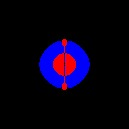
\includegraphics[width=\textwidth]{include/graphics/pml-off-0}
    \end{subfigure}
    ~
    \begin{subfigure}[b]{0.3\textwidth}
        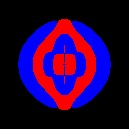
\includegraphics[width=\textwidth]{include/graphics/pml-off-1}
    \end{subfigure}
    ~
    \begin{subfigure}[b]{0.3\textwidth}
        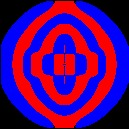
\includegraphics[width=\textwidth]{include/graphics/pml-off-2}
    \end{subfigure}
    
\bigskip
        \begin{subfigure}[b]{0.3\textwidth}
        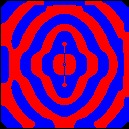
\includegraphics[width=\textwidth]{include/graphics/pml-off-3}
    \end{subfigure}
    ~
    \begin{subfigure}[b]{0.3\textwidth}
        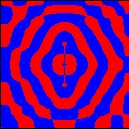
\includegraphics[width=\textwidth]{include/graphics/pml-off-4}
    \end{subfigure}
    ~
    \begin{subfigure}[b]{0.3\textwidth}
        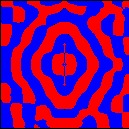
\includegraphics[width=\textwidth]{include/graphics/pml-off-5}
    \end{subfigure}

    \caption{Изменение электрического поля во времени (без PML)}\label{fig:EzPmlOff}
\end{figure}

\begin{figure}[p]
    \centering
%    \vspace{30mm}
    \begin{subfigure}[b]{0.3\textwidth}
        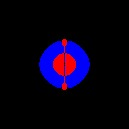
\includegraphics[width=\textwidth]{include/graphics/pml-on-0}
    \end{subfigure}
    ~
    \begin{subfigure}[b]{0.3\textwidth}
        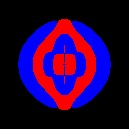
\includegraphics[width=\textwidth]{include/graphics/pml-on-1}
    \end{subfigure}
    ~
    \begin{subfigure}[b]{0.3\textwidth}
        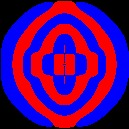
\includegraphics[width=\textwidth]{include/graphics/pml-on-2}
    \end{subfigure}
    
\bigskip
        \begin{subfigure}[b]{0.3\textwidth}
        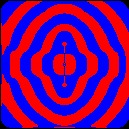
\includegraphics[width=\textwidth]{include/graphics/pml-on-3}
    \end{subfigure}
    ~
    \begin{subfigure}[b]{0.3\textwidth}
        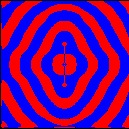
\includegraphics[width=\textwidth]{include/graphics/pml-on-4}
    \end{subfigure}
    ~
    \begin{subfigure}[b]{0.3\textwidth}
        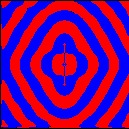
\includegraphics[width=\textwidth]{include/graphics/pml-on-5}
    \end{subfigure}

    \caption{Изменение электрического поля во времени (с PML)}\label{fig:EzPmlOn}
\end{figure}


\subsection{Перенос вычислительной нагрузки на графический процессор}

В целях увеличения производительности функции расчёта компонент векторов электрической и магнитной напряжённости были изменены
для исполнения на графических процессорах. Из двух технологий, позволяющих осуществить расчёт на GPU: NVIDIA CUDA и OpenCL --- была выбрана
вторая, так как она поддерживает процессоры не только производства компании NVIDIA, но и AMD.

Для облегчения работы с фреймворком OpenCL была использована библиотека EasyCL. Код расчёта компонент вектора магнитной напряжённости
приведён в приложении~Б. Зависимости среднего времени расчёта компонент векторов напряжённости в конкретный момент времени во всех ячейках от размеров сетки представлены на рис.~\ref{fig:1stComparsion} и~\ref{fig:2ndComparsion}.

\begin{figure}[p]
\centering
\captionsetup{justification=centering}
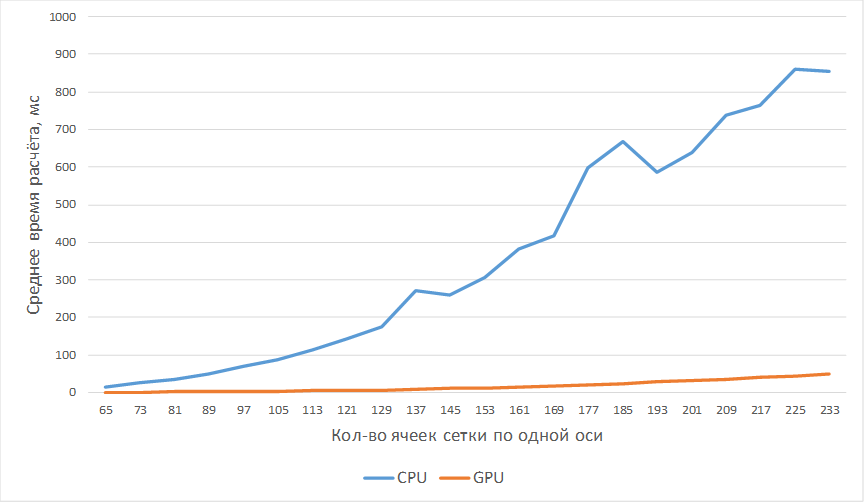
\includegraphics[width=0.95\textwidth]{include/graphics/image12}
\caption{Зависимость среднего времени расчёта компонент вектора $\vec{H}$ в конкретный момент времени во всех ячейках от размеров сетки}
\label{fig:1stComparsion}
\end{figure}
\begin{figure}[p]
\centering
\captionsetup{justification=centering}
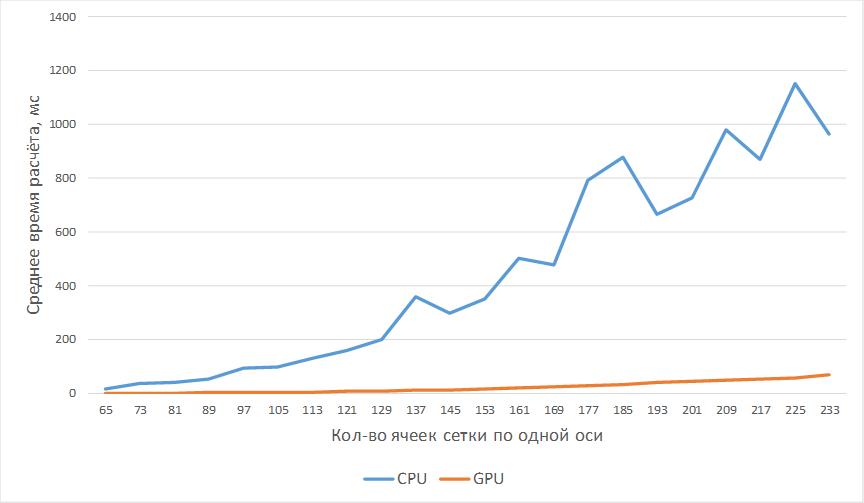
\includegraphics[width=0.95\textwidth]{include/graphics/image13}
\caption{Зависимость среднего времени расчёта компонент вектора $\vec{E}$ в конкретный момент времени во всех ячейках от размеров сетки}
\label{fig:2ndComparsion}
\end{figure}

\clearpage